%% tikz-slog.tex --- included by sensitivity_derivation.tex
%% Figure 1: the detection task. Panel (a) the geometry, panel (b) the two hypotheses
%% and their difference, the SLoG.
%% Requires: tikz, pgfplots (compat=1.18), subcaption, arrows.meta.

\begin{subfigure}[b]{0.53\textwidth}\centering
  \pgfmathsetmacro{\sA}{9}\pgfmathsetmacro{\sR}{2.2}\pgfmathsetmacro{\sAh}{\sA/2}
  \pgfmathsetmacro{\sw}{0.30}\pgfmathsetmacro{\se}{0.58}
  \pgfmathsetmacro{\seo}{\se*(\sR+\sw)/\sR}
  \pgfmathsetmacro{\rO}{1.15}\pgfmathsetmacro{\eO}{\se*\rO/\sR}
  \pgfmathsetmacro{\zz}{0.9}\pgfmathsetmacro{\dd}{\sAh-\zz}
  \pgfmathsetmacro{\zl}{\zz-\dd}
\begin{tikzpicture}[x=0.42cm,y=0.42cm,>={Latex[length=1.6mm]}]
  % detector cylinder: walls and far rim
  \fill[black!8] (-\sAh,\sR) rectangle (\sAh,{\sR+\sw});
  \fill[black!8] (-\sAh,{-\sR-\sw}) rectangle (\sAh,-\sR);
  \draw[black!45] (-\sAh,\sR) -- (\sAh,\sR);
  \draw[black!45] (-\sAh,{\sR+\sw}) -- (\sAh,{\sR+\sw});
  \draw[black!45] (-\sAh,-\sR) -- (\sAh,-\sR);
  \draw[black!45] (-\sAh,{-\sR-\sw}) -- (\sAh,{-\sR-\sw});
  % uniform attenuating cylinder, longer than the scanner
  \fill[cyan!8] (-\sAh-1.6,-\rO) rectangle (\sAh+1.6,\rO);
  \draw[cyan!40!black,opacity=0.45] (-\sAh-1.6,\rO) -- (\sAh+1.6,\rO);
  \draw[cyan!40!black,opacity=0.45] (-\sAh-1.6,-\rO) -- (\sAh+1.6,-\rO);
  \fill[cyan!14] (\sAh+1.6,0) ellipse ({\eO} and {\rO});
  \draw[cyan!40!black,opacity=0.45] (\sAh+1.6,0) ellipse ({\eO} and {\rO});
  \draw[black!30,densely dashed] (-\sAh,\sR)       arc ( 90:-90:{\se}  and {\sR});
  \draw[black!30,densely dashed] (-\sAh,{\sR+\sw}) arc ( 90:-90:{\seo} and {\sR+\sw});
  \draw[black!45] (-\sAh,\sR)       arc ( 90:270:{\se}  and {\sR});
  \draw[black!45] (-\sAh,{\sR+\sw}) arc ( 90:270:{\seo} and {\sR+\sw});
  % accepted solid angle at the position of the SLoG
  \fill[blue!12] (\zz,0) -- (\sAh,\sR)  -- (\zl,\sR)  -- cycle;
  \fill[blue!12] (\zz,0) -- (\sAh,-\sR) -- (\zl,-\sR) -- cycle;
  \draw[blue!65!black,line width=0.5pt] (\zl,-\sR) -- (\sAh,\sR);
  \draw[blue!65!black,line width=0.5pt] (\zl,\sR)  -- (\sAh,-\sR);
  % axis and near rim
  \draw[dash pattern=on 3pt off 1.5pt on 0.8pt off 1.5pt,black!55]
        (-\sAh-2.5,0) -- (\sAh+2.7,0) node[right,font=\tiny,black!60] {$z$};
  \draw[black!35,thin,densely dotted] (0,{-\sR-\sw}) -- (0,{\sR+\sw});
  \node[font=\tiny,black!45,anchor=north] at (0,{-\sR-\sw-0.05}) {$0$};
  \fill[black!8,even odd rule] (\sAh,0) ellipse ({\seo} and {\sR+\sw})
                               (\sAh,0) ellipse ({\se}  and {\sR});
  \draw[black!45] (\sAh,0) ellipse ({\seo} and {\sR+\sw});
  \draw[black!45] (\sAh,0) ellipse ({\se}  and {\sR});
  % the SLoG
  \foreach \rr/\oo in {0.44/0.12, 0.32/0.22, 0.21/0.40, 0.12/0.85}
    \fill[red!75!black,opacity=\oo] (\zz,0) circle (\rr);
  \node[font=\tiny,red!60!black,anchor=south west] at (\zz+0.30,0.32) {SLoG};
  % dimensions
  \draw[<->,black!70] (-\sAh-2.0,-\sR) -- (-\sAh-2.0,\sR)
        node[midway,fill=white,inner sep=1pt,font=\tiny] {$\Dpet$};
  \draw[<->,cyan!45!black] (\sAh+2.25,-\rO) -- (\sAh+2.25,\rO)
        node[midway,fill=white,inner sep=1pt,font=\tiny] {$\Dcyl$};
  \draw[<->,black!70] (-\sAh,{-\sR-\sw-0.75}) -- (\sAh,{-\sR-\sw-0.75})
        node[pos=0.30,fill=white,inner sep=1pt,font=\tiny] {$\Lpet$};
  \draw[black!35,thin,densely dotted] (\zz,-0.30) -- (\zz,{-\sR-\sw-0.40});
  \node[font=\tiny,anchor=north] at (\zz,{-\sR-\sw-0.18}) {$z$};
  \path (-\sAh-2.8,{-\sR-\sw-1.3}) rectangle (\sAh+2.9,{\sR+\sw+0.5});
\end{tikzpicture}
  \caption{The geometry.}
\end{subfigure}\hfill
\begin{subfigure}[b]{0.45\textwidth}\centering
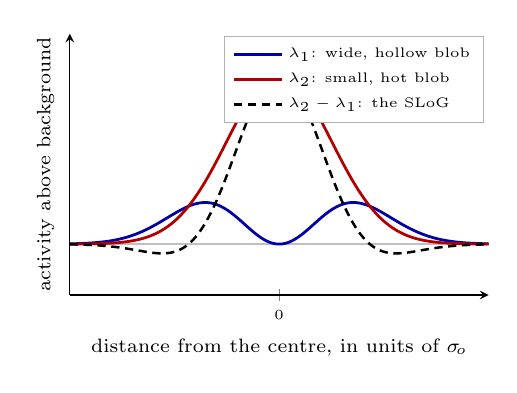
\begin{tikzpicture}
\begin{axis}[
  width=6.9cm, height=4.9cm,
  xmin=-4, xmax=4, ymin=-0.30, ymax=1.24,
  xlabel={distance from the centre, in units of $\sigma_{\!o}$}, ylabel={activity above background},
  ytick=\empty, xtick={0}, xticklabels={0},
  axis lines=left, enlargelimits=false,
  legend style={at={(0.99,0.99)},anchor=north east,font=\tiny,draw=black!30,
                legend cell align=left},
  tick label style={font=\tiny}, label style={font=\scriptsize},
]
  \addplot[black!25,line width=0.5pt,forget plot,domain=-4:4,samples=2] {0};
  \addplot[blue!65!black,line width=1pt,smooth,domain=-4:4,samples=250]
          {(x^2/3)*exp(-x^2/2)};
  \addlegendentry{$\lambda_1$: wide, hollow blob}
  \addplot[red!70!black,line width=1pt,smooth,domain=-4:4,samples=250]
          {exp(-x^2/2)};
  \addlegendentry{$\lambda_2$: small, hot blob}
  \addplot[black,densely dashed,line width=0.9pt,smooth,domain=-4:4,samples=250]
          {(1-x^2/3)*exp(-x^2/2)};
  \addlegendentry{$\lambda_2-\lambda_1$: the SLoG}
\end{axis}
\end{tikzpicture}
  \caption{The two hypotheses.}
\end{subfigure}
